\documentclass[12pt,a4paper]{article}

% --- Packages (same set and page setup as the Lab 1 report) ---
\usepackage[utf8]{inputenc}
\usepackage[T1]{fontenc}
\usepackage{lmodern}
\usepackage[english]{babel}
\usepackage[top=2.5cm,bottom=2.5cm,left=2.5cm,right=2.5cm]{geometry}
\usepackage{graphicx}
\usepackage{booktabs}
\usepackage{tabularx}
\usepackage{array}
\usepackage{float}
\usepackage{caption}
\usepackage{enumitem}
\usepackage{listings}
\usepackage{xcolor}
\usepackage{fancyhdr}
\usepackage[many]{tcolorbox}
\usepackage{microtype}
\usepackage{amsmath,amssymb}
\usepackage{tikz}
\usetikzlibrary{positioning,arrows.meta}
\usepackage{hyperref}

% --- Colours ---
\definecolor{primary}{RGB}{18,52,86}
\definecolor{secondary}{RGB}{41,128,185}
\definecolor{accent}{RGB}{231,76,60}
\definecolor{codebg}{RGB}{247,249,250}
\definecolor{codeframe}{RGB}{209,213,219}
\definecolor{codegray}{RGB}{108,117,125}
\definecolor{termgreen}{RGB}{80,250,123}
\definecolor{termred}{RGB}{255,85,85}
\definecolor{termyellow}{RGB}{241,250,140}

\hypersetup{colorlinks=true,linkcolor=primary,citecolor=secondary,urlcolor=secondary}

% --- Listings ---
\lstdefinestyle{code}{
    backgroundcolor=\color{codebg},
    basicstyle=\small\ttfamily,
    keywordstyle=\color{secondary}\bfseries,
    stringstyle=\itshape,
    commentstyle=\itshape\color{codegray},
    numbers=left,
    numberstyle=\tiny\color{codegray},
    numbersep=8pt,
    frame=single,
    rulecolor=\color{codeframe},
    breaklines=true,
    breakatwhitespace=true,
    showstringspaces=false,
    tabsize=4,
    captionpos=b
}
\lstdefinestyle{plain}{
    backgroundcolor=\color{codebg},
    basicstyle=\small\ttfamily,
    frame=single,
    rulecolor=\color{codeframe},
    breaklines=true,
    showstringspaces=false,
    captionpos=b
}
\lstdefinestyle{term}{
    backgroundcolor=\color{codebg},
    basicstyle=\small\ttfamily,
    frame=single,
    rulecolor=\color{codeframe},
    breaklines=true,
    showstringspaces=false,
    captionpos=b
}

% --- Terminal window (as in the Lab 1 report) ---
\tcbuselibrary{listings,skins}
\newtcblisting{terminalwindow}[1][]{%
    enhanced,
    colback=black,
    colframe=black,
    arc=2.5mm,
    boxrule=1pt,
    title={\textcolor{termred}{$\bullet$}\;\textcolor{termyellow}{$\bullet$}\;\textcolor{termgreen}{$\bullet$}\quad \textsf{\bfseries Console Terminal Session}},
    fonttitle=\small\sffamily\bfseries,
    coltitle=white,
    attach boxed title to top left={yshift=-2mm, xshift=4mm},
    boxed title style={colback=gray!15!black, arc=1.5mm, boxrule=0.5pt},
    listing only,
    listing options={
        backgroundcolor=\color{black},
        basicstyle=\small\ttfamily\color{white},
        frame=none,
        numbers=none,
        breaklines=true,
        tabsize=4,
        showspaces=false,
        showstringspaces=false,
        keepspaces=true
    },
    #1
}

% --- Header and footer: page number only, no header rule ---
\lstset{style=plain}

\pagestyle{fancy}
\fancyhf{}
\setlength{\headheight}{15pt}
\addtolength{\topmargin}{-3pt}
\fancyfoot[C]{\thepage}
\renewcommand{\headrulewidth}{0pt}
\renewcommand{\footrulewidth}{0pt}

\newcommand{\studentgroup}{FAF-241}

\begin{document}
\setlength{\emergencystretch}{2em}

\begin{titlepage}
    \centering
    {\large \textbf{TECHNICAL UNIVERSITY OF MOLDOVA}}\\[0.2cm]
    {\large Faculty of Computers, Informatics and Microelectronics}\\[0.2cm]
    {\large Department of Software Engineering and Automatics}\\[0.8cm]

    
\includegraphics[width=3.5cm]{figures/utm_logo.png}\\[1.2cm]

    {\Large \textbf{LABORATORY WORK NO. 2}}\\[0.4cm]
    {\LARGE \textbf{A Coffee Shop Server:\\ TCP Sockets, Worker Threads, and Shared State}}\\[0.4cm]
    {\large Course: Network Programming}\\[2.5cm]

    \begin{minipage}{0.52\textwidth}
        \flushleft
        \textbf{Authors:}\\
        Dinu \textsc{Plesu}\\
        Igor \textsc{Boltunov}\\
        Student group: \studentgroup
    \end{minipage}
    \hfill
    \begin{minipage}{0.40\textwidth}
        \flushright
        \textbf{Verified by:}\\
        Lecturer / Supervisor\\
        Fistic Cristofor
    \end{minipage}

    \vfill
    {\large Chi\c{s}in\u{a}u --- 2026}
\end{titlepage}

\newpage
\newpage
\tableofcontents
\newpage

\section{Introduction}
\label{sec:intro}

\subsection{Motivation and problem statement}

A concurrent TCP server is a compact testbed for three classic systems problems:
turning a byte stream into messages, coordinating producers and consumers through
a shared queue, and protecting shared state from race conditions. TCP delivers a
reliable, ordered byte stream but no message boundaries, so the
application must define its own framing and validation. The correctness of the
last item in a shared stock depends on a critical section, not on timing. When a
client disappears, the server has to reclaim that client's orders and products
without stopping the other clients.

The coffee-shop task combines these concerns. The server has three roles
(server, client, provider), a fixed worker pool, a shared stock, and failure
handling for clients and the provider. The task also offers three bonuses: two
computers, two programming languages, and a stock that survives a restart. All
three are implemented and evaluated here.

\subsection{Task map}

Table~\ref{tab:taskmap} connects each task of the laboratory sheet to the
design section that implements it and the section that reports its evidence.

\begin{table}[H]
\centering
\small
\begin{tabularx}{\textwidth}{@{}l X l l@{}}
\toprule
Task & Requirement in the sheet & Design & Evidence \\
\midrule
1. One client & menu, order, refusal, ready message, errors & \S\ref{sec:design} & \S\ref{sec:task1} \\
2. Many clients & shared stock, FIFO queue, one worker per processor & \S\ref{sec:design} & \S\ref{sec:task2} \\
3. The provider & deliveries, low-stock alerts, provider reconnect & \S\ref{sec:design} & \S\ref{sec:task3} \\
4. When things go wrong & disconnects, invalid input, live output & \S\ref{sec:design} & \S\ref{sec:task4} \\
Bonuses & two computers, two languages, stock persistence & \S\ref{sec:design} & \S\ref{sec:bonus} \\
\bottomrule
\end{tabularx}
\caption{Map from the laboratory sheet to the sections of this report.}
\label{tab:taskmap}
\end{table}

\subsection{Objectives}

The objectives are:
\begin{enumerate}[itemsep=1pt]
    \item implement a TCP server that accepts many clients and a provider using
          the socket API directly, without \texttt{TcpListener}, \texttt{TcpClient},
          or \texttt{NetworkStream};
    \item implement the menu, order, refusal, preparation, and ready notification
          semantics of the coffee shop;
    \item create one worker per logical processor, a FIFO order queue, and a stock
          protected against concurrent access;
    \item alert the provider when a product falls below five units, including on
          provider reconnect;
    \item cancel and refund the orders of a client that disappears, while keeping
          the server available to the others;
    \item persist the stock across a restart and evaluate the server on two
          computers and in two languages.
\end{enumerate}

\section{Background}
\label{sec:background}

\subsection{TCP and socket programming}

TCP provides a reliable, ordered byte stream between two endpoints
. It handles retransmission, flow control, and connection setup,
but it does not keep application message boundaries. A server that reads from a
socket may receive half a message, two messages, or the end of one message
followed by the start of the next. The application must therefore buffer bytes,
find a delimiter or a length prefix, and validate what it finds. This work uses
newline-delimited JSON: each message is one JSON object followed by a newline,
and a line that is too long is rejected.

The socket API exposes the sequence \texttt{socket}, \texttt{bind},
\texttt{listen}, \texttt{accept}, \texttt{send}, \texttt{receive}, and
\texttt{close}. The listening socket carries no data; each accepted connection has
its own socket and its own reader thread. A thread per connection is simple and
direct, but it costs a stack and a context switch per client. Section~\ref{sec:control}
returns to this trade-off.

\subsection{Producer--consumer systems and worker pools}

The server is a producer--consumer system. Connection threads are the producers:
they validate an order, take its products from the stock, and put the order in a
queue. Workers are the consumers: each takes the oldest order and simulates its
preparation. The pattern decouples request handling from the duration of the
work and is a standard operating-systems example. A fixed
worker pool bounds the number of orders prepared at the same time, and a FIFO
queue preserves arrival order when every worker is busy.

\subsection{Shared state and race conditions}

The stock is shared mutable state. A check followed by a decrement is not atomic
by default: two threads can both observe the last item and both accept an order
. The server therefore performs the stock check and the decrement
inside one critical section protected by a lock. The same reasoning applies to
the order identifier counter, the session and provider lists, and the metrics
counters. A second kind of shared state is the connection itself: reader threads,
workers, and alert senders may all write to the same session, so every session
has a write lock and every message is written as one complete line.

\subsection{Performance measures and queueing}

The evaluation uses queue wait, preparation time, throughput, and per-worker
utilisation. Little's law relates the average number of items in a system to the
arrival rate and the average time in the system, $L=\lambda W$.
Amdahl's law bounds the speed-up from adding workers when part of the work is
serial. In this laboratory the preparation is simulated by waiting,
so the workers are mostly idle from the processor's point of view. The
measurements therefore describe scheduling and queueing, not CPU-bound work.

\subsection{Positioning}

The implementation is deliberately small. It does not use an asynchronous event
loop, a thread-pool library, or a web framework, because those would hide the
socket and concurrency mechanisms that the laboratory asks students to understand.
The C\#, Go, and Rust programs share one wire protocol. The measured runs use the
C\# server with Go clients and the C\# client; the Go server was tested for
persistence; the Rust programs are in the repository but were not part of the
measurements.

\section{System Design}
\label{sec:design}

\subsection{System model and notation}

Let $O$ be the set of orders. An order $o\in O$ asks for $q_{o,i}$ units of each
product $i$. Each product has a fixed preparation time per unit, $p_i$: coffee
4~s, tea 3~s, croissant 2~s. The nominal preparation time of an order is
\begin{equation}
T_{\mathrm{prep}}(o) = \sum_{i} q_{o,i}\,p_i.
\label{eq:prep}
\end{equation}
An order is accepted only if the stock $s_i$ satisfies $s_i\ge q_{o,i}$ for every
product, and the check and the decrement form one critical section:
\begin{equation}
\text{accept}(o) \iff \forall i:\; s_i \ge q_{o,i},
\qquad
s_i \leftarrow s_i - q_{o,i}.
\label{eq:stock}
\end{equation}

With $W$ workers, a FIFO queue, and $N_{\mathrm{ready}}$ finished orders in a run
of length $T_{\mathrm{run}}$, the throughput and the utilisation of worker $w$ are
\begin{equation}
X = \frac{N_{\mathrm{ready}}}{T_{\mathrm{run}}},
\qquad
U_w = \frac{B_w}{T_{\mathrm{run}}},
\label{eq:throughput}
\end{equation}
where $B_w$ is the time that worker $w$ spent preparing orders. The server metrics
report exactly these quantities.

\begin{figure}[H]
\centering
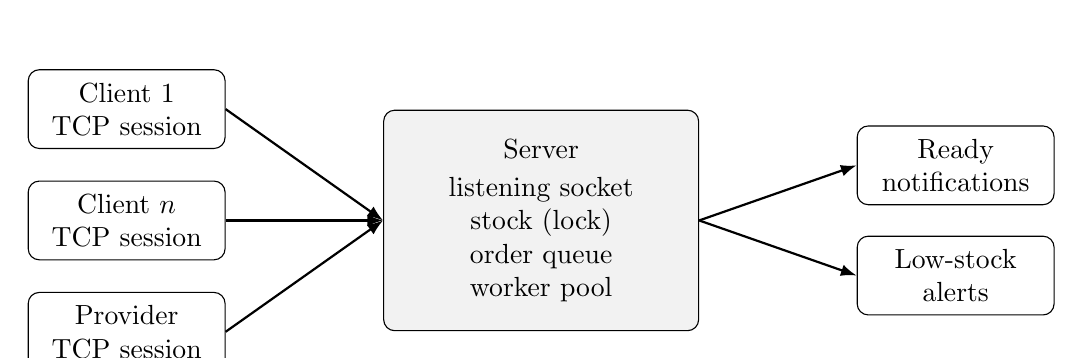
\begin{tikzpicture}[
  node distance=1.6cm,
  box/.style={draw, rounded corners, minimum width=2.5cm, minimum height=1.0cm,
              align=center, fill=white},
  server/.style={draw, rounded corners, minimum width=4.0cm, minimum height=2.8cm,
                 align=center, fill=gray!10},
  arrow/.style={-{Latex[length=2mm]}, thick}
]
\node[box] (c1) {Client 1\\TCP session};
\node[box, below=0.4cm of c1] (c2) {Client $n$\\TCP session};
\node[box, below=0.4cm of c2] (prov) {Provider\\TCP session};
\node[server, right=2.0cm of c2] (srv)
  {Server\\[2pt]listening socket\\stock (lock)\\order queue\\worker pool};
\node[box, right=2.0cm of srv, yshift=0.7cm] (ready) {Ready\\notifications};
\node[box, right=2.0cm of srv, yshift=-0.7cm] (alerts) {Low-stock\\alerts};
\draw[arrow] (c1.east) -- (srv.west);
\draw[arrow] (c2.east) -- (srv.west);
\draw[arrow] (prov.east) -- (srv.west);
\draw[arrow] (srv.east) -- (ready.west);
\draw[arrow] (srv.east) -- (alerts.west);
\end{tikzpicture}
\caption{Server model. The listening socket creates one session per connection.
The stock and the FIFO order queue are protected by locks, and the worker pool
consumes orders and sends ready notifications.}
\label{fig:server-model}
\end{figure}

\subsection{Roles and sockets}

The server binds one listening socket to \texttt{0.0.0.0:5000}, calls
\texttt{Listen} once, and then calls \texttt{Accept} repeatedly. Each accepted
connection gets its own socket and its own reader thread. The reader parses
commands, updates the shared state under locks, answers the client, and, when an
order is accepted, puts it in the work queue.

The client and the provider are the same program. After connecting, the first
message names the role:

\begin{lstlisting}[style=plain,caption={Handshake sent by the client or the provider.}]
{"cmd":"hello","role":"client"}
{"cmd":"hello","role":"provider"}
\end{lstlisting}

\subsection{Framing and protocol}

TCP is a byte stream: one \texttt{send} is not one \texttt{receive}. The server
keeps a string buffer, appends every received chunk, and handles every complete
line. A line longer than 4096 characters (bytes in the Go server) gets a
\texttt{message too long} error and is skipped. If the C\# buffer grows beyond
four times that limit without a newline, the server sends the error and closes
the connection, so a client cannot make the server allocate without bound.

Every message is one JSON object. Table~\ref{tab:protocol} lists the commands.

\begin{table}[h]
\centering
\small
\begin{tabularx}{\textwidth}{@{}l l X@{}}
\toprule
Direction & Message & Meaning \\
\midrule
client $\rightarrow$ server & \texttt{hello} & identify as client or provider \\
client $\rightarrow$ server & \texttt{menu} & request the products and the stock \\
client $\rightarrow$ server & \texttt{order} & order a list of products and quantities \\
provider $\rightarrow$ server & \texttt{deliver} & add products to the stock \\
client $\rightarrow$ server & \texttt{stats} & request the live server summary \\
client $\rightarrow$ server & \texttt{quit} & close the connection \\
\midrule
server $\rightarrow$ client & \texttt{menu} & current stock \\
server $\rightarrow$ client & \texttt{order\_accepted} & order id, preparation time, tag \\
server $\rightarrow$ client & \texttt{order\_refused} & product and how many are left \\
server $\rightarrow$ client & \texttt{order\_ready} & order id is ready \\
server $\rightarrow$ provider & \texttt{alert} & low stock (provider only) \\
server $\rightarrow$ provider & \texttt{delivery\_ok} & delivery accepted \\
server $\rightarrow$ client & \texttt{stats} & connections, orders, averages \\
server $\rightarrow$ client & \texttt{error} & invalid command or parameter \\
\bottomrule
\end{tabularx}
\caption{The line-delimited JSON protocol.}
\label{tab:protocol}
\end{table}

An order is answered at once, and readiness comes later as a separate message:

\begin{lstlisting}[style=plain,caption={An order is accepted at once; readiness arrives later.}]
{"cmd":"order","items":[{"product":"coffee","qty":1}]}
{"type":"order_accepted","id":3,"prep":4000,"tag":0}
...
{"type":"order_ready","id":3,"tag":0}
\end{lstlisting}

\subsection{Workers, queue and shared state}

At startup the server creates one worker per logical processor: the C\# server
reads \texttt{Environment.ProcessorCount} and the Go server reads
\texttt{runtime.NumCPU()}. On the desktop used as the server this gives 12 (an
Intel Core i5-13420H with 8 cores and 12 threads), and the log says
\texttt{Started 12 workers}.

Connection threads are the producers. They validate an order, take its products
from the stock at once, and put the order in a FIFO blocking queue of
\texttt{Order} objects. Workers are the consumers: a free worker takes the oldest
order and simulates its preparation by waiting. The shared objects and their
protection are:

\begin{itemize}[itemsep=2pt]
    \item the stock (coffee, tea, croissant), protected by \texttt{StockLock}: the
          check and the decrement happen in one critical section, so the last
          croissant cannot be sold twice;
    \item the order identifier counter, protected by \texttt{IdLock};
    \item the list of sessions and the provider list, protected by \texttt{SessionsLock};
    \item each connection, which is written from several threads (the reader's
          answers, the worker's readiness messages, alerts), has its own write lock;
    \item each order's \texttt{Claimed} flag, changed with an atomic
          compare-and-exchange (see Disconnects and cancellation below);
    \item the metrics counters, protected by the metrics lock.
\end{itemize}

\subsection{Provider, deliveries and alerts}

The provider is an ordinary connection whose \texttt{hello} names the provider
role. The server keeps it in a separate list. A delivery is validated and added to
the stock in one critical section. A client that sends \texttt{deliver} receives
\texttt{only provider can deliver}.

After every accepted order, delivery, and refund, the server checks the stock. The
check reads the stock under \texttt{StockLock}, releases the lock, and then sends
an \texttt{alert} to every connected provider for each product below 5. When a
provider connects, its own connection thread sends the current low-stock products
right after the \texttt{hello}. Without this step, a provider that was offline would
never learn that the shop was almost empty.

\subsection{Disconnects and cancellation}

Every order has a cancellation token and a \texttt{Claimed} flag. The flag is 0
while the order waits in the queue and becomes 1 when a worker starts it or when
it is cancelled while queued. The reader thread notices a closed connection when
\texttt{Receive} returns 0 (an orderly close) or fails with a reset (an aborted
connection). It then cancels every token of that client and tries to set
\texttt{Claimed} from 0 to 1 for each order:

\begin{itemize}[itemsep=2pt]
    \item if the exchange succeeds, no worker has started the order, so the reader
          returns its products to the stock at once; a worker that later dequeues
          the order sees \texttt{Claimed = 1} and skips it;
    \item if the exchange fails, a worker already owns the order. The worker checks
          the token in steps of at most 100~ms, stops when it sees the cancellation,
          returns the products to the stock under \texttt{StockLock}, logs the refund,
          and continues with the next order.
\end{itemize}

The products return to the stock. The time already spent preparing them is lost,
so the next order that takes them waits the full preparation again.

A provider that disappears is removed from the provider list, the stock stays as
it is, and the server keeps serving clients. Invalid input (an unknown command,
wrong parameters, a line that is too long, random bytes) gets an \texttt{error}
answer, is logged as \texttt{Error to <endpoint>: <reason>}, and does not stop the
server.

\subsection{Metrics}

The server appends one row to \texttt{server-orders.csv} for each finished order
(order id, endpoint, items, expected and actual preparation, queue wait, worker
id, status). It rewrites \texttt{server-summary.json} every two seconds with the
connections, the accepted, refused, ready, and cancelled orders, deliveries,
alerts, averages, throughput, and per-worker orders, busy time, and utilisation.

Each C\# client writes \path{client-orders-<pid>.csv} and
\path{client-summary-<pid>.json}. The files are per process, so several clients
can run at once without writing to the same file. The Python script
\path{Lab2/scripts/metrics_report.py} uses only the standard library. It merges
the CSV files and writes \texttt{report.md} and SVG charts. The figures in this
report are the same charts exported as PNG.

\subsection{Stock persistence}

The stock is written to \texttt{stock-state.json} in the server's working
directory after every accepted order, delivery, and cancellation refund. The write
is atomic: a snapshot is taken under the stock lock, written to a temporary file,
and renamed over the old file. At startup the server loads the file, validates
that all three products are present with non-negative counts, and logs the result:

\begin{terminalwindow}[]
[06:16:22.563] Stock loaded from stock-state.json: coffee=20, tea=19, croissant=21
[06:16:22.573] Started 12 workers
[06:16:22.577] Listening on 0.0.0.0:5000
\end{terminalwindow}

A missing or corrupt file is rejected as a whole, and the server starts with a
random stock of 10 to 50 units of each product. The bonus is implemented in the C\#
and the Go server.

\section{Evaluation Setup}
\label{sec:setup}

\subsection{Procedure}

The procedure is:
\begin{enumerate}[itemsep=1pt]
    \item build the C\# server and client with the commands in Section~\ref{sec:source};
    \item start a fresh C\# server with a random stock and 12 workers;
    \item run one client, the invalid-input checks, the last-item race, the
          provider, the alerts, and a mid-order disconnect;
    \item run 16 Go clients and a provider from a phone (earlier run) and from a
          second desktop, with the server metrics enabled;
    \item run five C\# clients on the server desktop to obtain client-side latency;
    \item stop and restart the server to verify stock persistence, for the C\# and the Go server;
    \item parse the server and client files and generate the tables and charts with
          \path{Lab2/scripts/metrics_report.py}.
\end{enumerate}

The unit of analysis is one finished order row in the server CSV, or one line of a
client transcript. The measures are descriptive: the report gives averages and
maxima, not confidence intervals.

\subsection{Environment}

\begin{table}[H]
\centering
\small
\begin{tabularx}{\textwidth}{@{}l X@{}}
\toprule
Role / owner & Machine and environment \\
\midrule
Server (desktop A) & \textbf{Dinu Plesu}: HP OMEN 16-wd0xxx; Windows 11 IoT Enterprise LTSC 10.0.26300, 64-bit; Intel Core i5-13420H, 8 cores / 12 threads, 2.1 GHz; 16 GB DDR5-5600; NVMe storage; Wi-Fi 6E, 192.168.1.41 in the two-desktop run \\
Clients (desktop B) & \textbf{Igor Boltunov}: CachyOS Linux, kernel 7.3.6-1-cachyos, x86-64; Intel Core i5-10300H, 4 cores / 8 threads, 2.5--4.5 GHz; 7.6 GiB RAM; Wi-Fi 6, 192.168.1.22 \\
Phone (earlier run) & Android, arm64 Go binaries (Acode/Alpine userland), Wi-Fi 192.168.1.5 \\
Runtimes &.NET 10.0.404; Go 1.27.4; Rust 1.99.1; Python 3.15.2 (Windows) / 3.14.10 (Linux) \\
\bottomrule
\end{tabularx}
\caption{Test environment: both authors' machines and the phone.}
\label{tab:env}
\end{table}

Both desktops were on the same Wi-Fi network. The phone clients connected to the
server at \texttt{192.168.1.33:5000}, and the two-desktop clients connected to
\texttt{192.168.1.41:5000}.

\subsection{What the evidence covers}

Every number in Sections~\ref{sec:task1} to~\ref{sec:bonus} comes from a run whose
files are in the repository (Section~\ref{app:evidence}), with two kinds of exception
that the text marks. First, the 20-client run, the last-item race, the mid-order
disconnect, the provider disconnect, and the server-death exit were run by hand during
development. Their results are recorded in \texttt{Lab2/KNOWLEDGE.md}, but no transcript
is archived. Second, the invalid-input checks and the low-stock alert are listed in the
defence checklist \path{docs/tutorials/02-testing.md}, but no run records their result:
every archived server summary reports \texttt{alerts = 0} and \texttt{errors = 0}. Those
two paths are therefore described from the code.

\section{Task 1: One Client}
\label{sec:task1}

The sheet asks for the menu, one order at a time, a refusal that tells the client
how many units are left, an immediate answer with the order number and the
preparation time, a later ready message, and an error for an unknown product or a
quantity that is not positive.

\subsection{Results}

A C\# client connected, asked for the menu, ordered one coffee, and waited. Its
transcript (\path{Lab2/evidence/stock-persistence-2026-11-26/client-order.txt})
shows the menu \texttt{coffee=21 tea=19 croissant=21}, the answer
\texttt{Order 1 accepted, prep 4000 ms}, and then \texttt{Order 1 READY} when the
worker finished. The client stayed usable while it waited, because its receive
thread prints server messages as they arrive while the main thread keeps reading
the keyboard (Section~\ref{sec:task4}).

Refusal is shown by the last-item race of Task~2: a refused order returns the
product and \texttt{available}, the number left. Invalid input (an unknown product,
a zero or negative quantity, a missing parameter, random bytes, a line that is too
long) is answered with an \texttt{error} message and logged with the endpoint. These
defence checklist (\path{docs/tutorials/02-testing.md}) lists these checks, but no run
records their result, so this paragraph describes the code path.

\subsection{Defence questions}

    \subsubsection{Q1. How does your code cut the received bytes into messages? What happens when a message arrives in two pieces, or two messages arrive in one receive?}
    The server appends each received chunk to a string buffer and repeatedly searches
    it for a newline. Every complete line is removed from the buffer and handled, so
    one receive can contain several messages. A message split across receives waits
    in the buffer until its newline arrives. A line longer than 4096 characters gets
    a \texttt{message too long} error and is skipped.

    \subsubsection{Q2. Why does the server answer at once and tell the client later that the order is ready? What would the client see otherwise?}
    The preparation takes 4 s for a coffee and up to 6 s for three croissants. If the
    server kept the answer until the order was ready, the client would see nothing for
    that time and could not order again or ask for the menu. The order number is sent
    immediately, so the client can match the later \texttt{order\_ready} message to it
    by the id and the tag.

\section{Task 2: Many Clients}
\label{sec:task2}

The sheet asks for many clients connected at the same time, a free worker that
takes the oldest waiting order, clients that keep ordering while they wait, and a
guarantee that two clients cannot both get the last croissant. It asks for a
demonstration with more clients than workers.

\subsection{Results}

\paragraph{Five clients, no queueing.} Two runs had five C\# clients ordering at the
same time against the desktop server with 12 workers. In both, all five orders were
accepted and became ready at once, so the queue wait was zero. The first run
(\path{cross-device-2026-11-26/desktop-csharp-clients-metrics/}) measured an average
acceptance latency of 6.6~ms and an average wait for readiness of 5901.2~ms. The
second run (\path{two-desktop-2026-11-26/windows-csharp-clients-metrics/}) measured
9.0~ms and 4197.6~ms. The acceptance latency is the time for one request and its
answer; the readiness wait is the preparation.

\paragraph{More clients than workers (phone).} The provider and 16 Go clients ran
on the phone against the C\# server on the desktop. With 12 workers, the first 12
orders started at once. The other four waited for a free worker, which is the FIFO
behaviour the sheet asks for. Table~\ref{tab:cross} summarises the run, and
Figure~\ref{fig:queue} shows the queue wait per order. Orders 11, 13, and 14 waited
about 4.4~s, and order 12 waited 6.6~s. Figure~\ref{fig:workers} shows which worker
prepared each order: four workers prepared two orders and the other eight prepared
one.

\begin{table}[h]
\centering
\small
\begin{tabularx}{\textwidth}{@{}X r@{}}
\toprule
Metric & Value \\
\midrule
Workers & 12 \\
Connections (16 clients + 1 provider) & 17 \\
Orders accepted / ready / refused / cancelled & 16 / 16 / 0 / 0 \\
Deliveries & 1 \\
Average queue wait & 1229.8 ms \\
Maximum queue wait & 6563.9 ms \\
Average actual preparation & 5748.3 ms \\
Maximum actual preparation & 6592.8 ms \\
Throughput & 0.57 orders/s \\
\bottomrule
\end{tabularx}
\caption{Phone run: 16 Go clients on an Android phone, 12 workers on the desktop server.}
\label{tab:cross}
\end{table}

\begin{figure}[h]
\centering
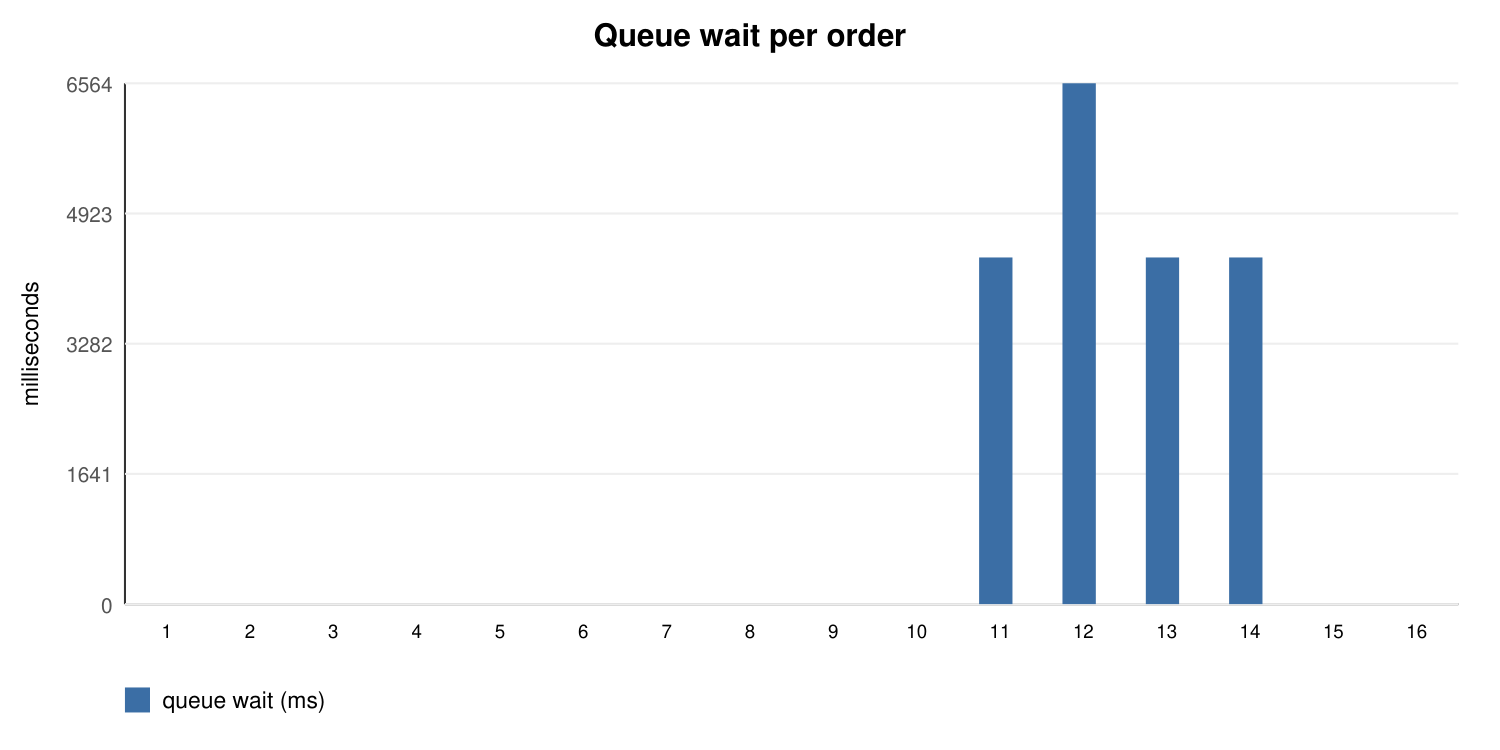
\includegraphics[width=0.95\linewidth]{figures/queue_wait.png}
\caption{Queue wait per order in the phone run. Twelve orders started at once. Orders
11, 13, and 14 waited about 4.4~s for a free worker, and order 12 waited 6.6~s.}
\label{fig:queue}
\end{figure}

\begin{figure}[h]
\centering
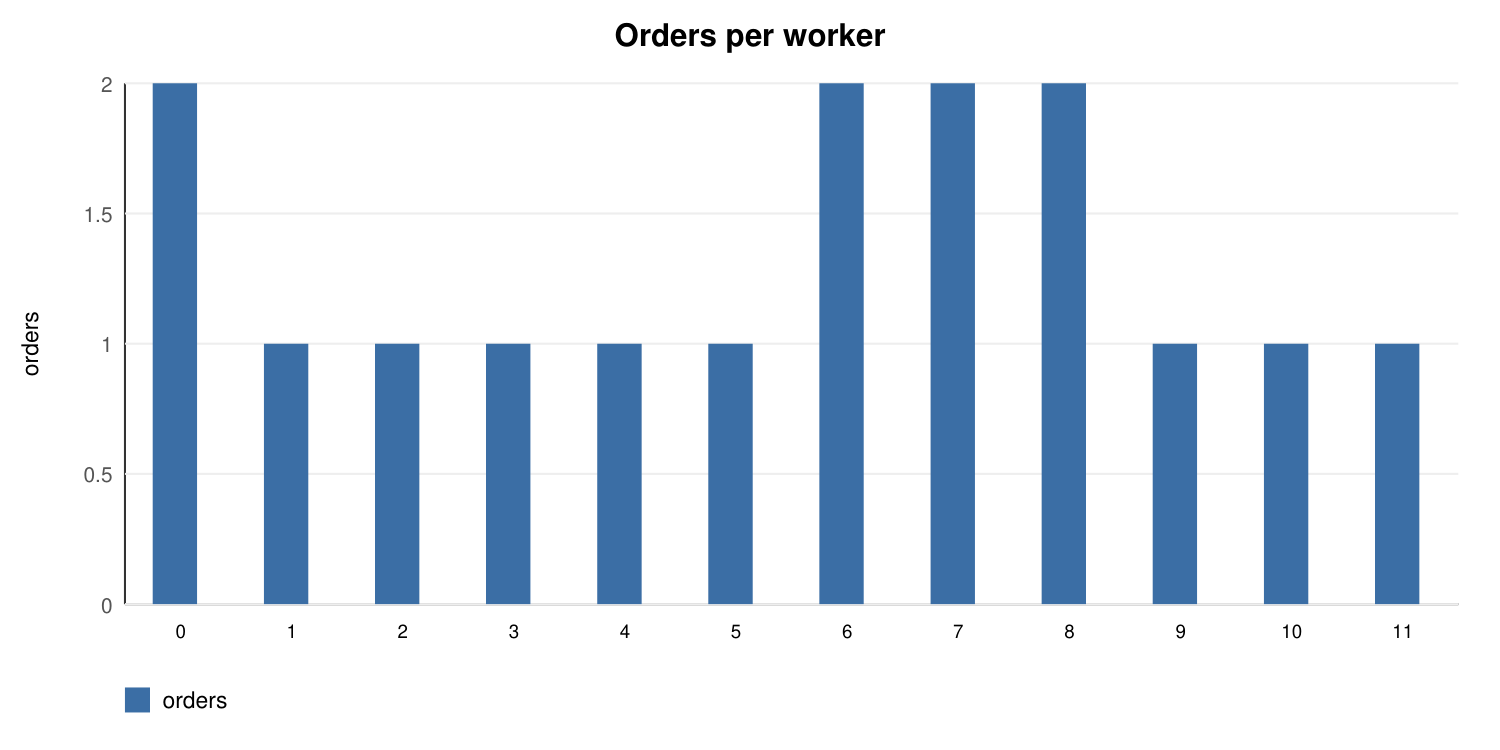
\includegraphics[width=0.95\linewidth]{figures/worker_orders.png}
\caption{Orders prepared by each worker in the phone run. Workers 0, 6, 7, and 8
prepared two orders each; the other eight prepared one.}
\label{fig:workers}
\end{figure}

\begin{figure}[h]
\centering
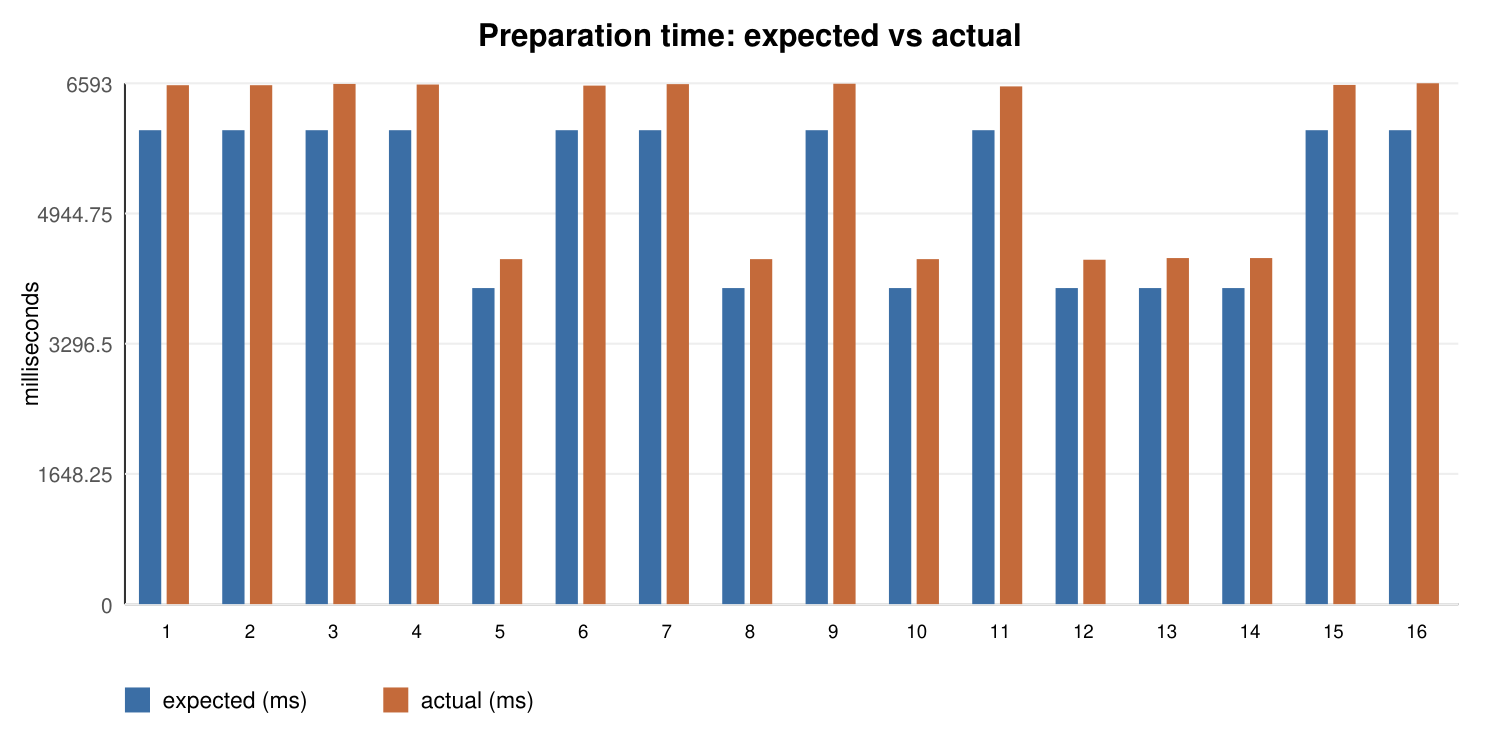
\includegraphics[width=0.95\linewidth]{figures/prep_time.png}
\caption{Expected and actual preparation time per order in the phone run. The actual
time is 0.36 to 0.59~s longer than the nominal time (Section~\ref{sec:discussion}).}
\label{fig:prep}
\end{figure}

\paragraph{More clients than workers (two desktops).} The provider delivered
\texttt{coffee:40 tea:40 croissant:40}, and 16 Go clients on the second desktop
ordered at the same time. All 16 orders were accepted and all 16 became ready. Four
orders (13 to 16) waited about 4.19~s each for a worker, and the other twelve started
at once. Table~\ref{tab:twodesktop} gives the server summary from the run's
\texttt{server-summary.json}. The charts and the 16 transcripts are in
\path{two-desktop-2026-11-26/}.

\begin{table}[H]
\centering
\small
\begin{tabularx}{\textwidth}{@{}X r@{}}
\toprule
Metric & Value \\
\midrule
Workers & 12 \\
Connections (16 clients + 1 provider) & 17 \\
Orders accepted / ready / refused / cancelled & 16 / 16 / 0 / 0 \\
Average queue wait & 1048.5 ms \\
Maximum queue wait & 4194.4 ms \\
Average actual preparation & 4213.9 ms \\
Maximum actual preparation & 4241.5 ms \\
Throughput & 0.44 orders/s \\
\bottomrule
\end{tabularx}
\caption{Two-desktop run: 16 Go clients on a CachyOS desktop, 12 workers on the Windows desktop.}
\label{tab:twodesktop}
\end{table}

\paragraph{Other manual run.} \texttt{Lab2/KNOWLEDGE.md} records a run with 20 clients
against 12 workers in which all 20 orders were accepted and became ready. No transcript
is archived.

\paragraph{The last-item race.} With one croissant left, two clients ordered it at
the same moment. The \texttt{StockLock} critical section accepted exactly one order
and refused the other with \texttt{available: 0}. This result is recorded in
\texttt{Lab2/KNOWLEDGE.md} and was not archived as a transcript.

\subsection{Defence questions}

    \subsubsection{Q1. Which data is shared between threads in your server, and how is each of them protected?}
    The stock is protected by \texttt{StockLock}, which makes the check and the
    decrement one step. The order id counter is protected by \texttt{IdLock}. The
    session list and the provider list are protected by \texttt{SessionsLock}. Each
    connection has a write lock, so two threads cannot interleave the bytes of two
    answers. The metrics counters have their own lock. Each order's \texttt{Claimed}
    flag is changed with an atomic compare-and-exchange, so a worker and the disconnect
    handler cannot both take the same order.

    \subsubsection{Q2. Two clients order the last croissant at the same moment. Show, step by step, what could go wrong without your protection.}
    Let the stock hold one croissant. Thread A (client 1) reads the stock and sees 1,
    so the order may proceed. Thread B (client 2) reads the stock before A writes
    anything and also sees 1. A decrements the stock to 0 and accepts. B decrements
    the stock to $-1$ and also accepts. Both clients receive a croissant, and the
    stock is negative. With \texttt{StockLock}, A takes the lock, checks $1 \ge 1$,
    decrements to 0, and releases the lock. B then takes the lock, checks $0 \ge 1$,
    fails, and is refused with \texttt{available: 0}.

    \subsubsection{Q3. A worker tells a client that its order is ready while the thread of that client is reading from the same connection. What must you take care of?}
    Reading and writing on one socket are independent, so the reader can keep receiving
    while a worker writes. What must be protected is the writing: two threads writing at
    the same time could interleave the bytes of two JSON lines. Each session therefore
    has a write lock, and every message is written as one complete line while the lock
    is held.

    \subsubsection{Q4. Why one worker per CPU core? The workers spend their time waiting: what would happen with twice as many?}
    The sheet fixes the capacity of the shop at one worker per logical processor, so at
    most that many orders are prepared at the same time. In this lab a worker mostly
    waits, so twice as many workers would cost little CPU and would raise the peak
    throughput roughly in proportion, as long as orders were waiting. The shop would
    then prepare more orders at once than the machine has processors, which is not the
    shop the sheet describes. For a CPU-bound preparation, more workers than cores would
    add only context switches and memory, with no extra parallelism.

\section{Task 3: The Provider}
\label{sec:task3}

The sheet asks that only the provider can deliver products, that the server alert
the provider when a product falls below five, and that the alert be sent without a
request, including to a provider that connects later.

\subsection{Results}

The provider identified itself with \texttt{hello}, and the server logged
\texttt{Provider identified: 192.168.1.5:56146}. Its delivery was added to the stock
at once and logged as \texttt{Delivery from 192.168.1.5:56146: coffee=40,tea=40,croissant=40},
followed by a \texttt{delivery\_ok} answer. The two-desktop run had the same delivery
(\texttt{coffee:40 tea:40 croissant:40}). A client that tried to deliver received
\texttt{only provider can deliver}, and the server logged the refusal.

The alert path is implemented as described in Section~\ref{sec:design}: the server
checks the stock after every order, delivery, and refund, and sends an \texttt{alert}
for each product below 5. A provider that connects receives the current low-stock
products right after its \texttt{hello}. The requirements matrix marks the alert as
passing on the strength of the code, and the defence checklist
(\path{docs/tutorials/02-testing.md}) lists the test. No run records an alert
(\texttt{alerts = 0} in every summary), so this result has no archived transcript.

\subsection{Defence questions}

    \subsubsection{Q1. How does your server know which connection is the provider?}
    The provider sends \texttt{hello} with \texttt{role:"provider"}. The server marks
    that session, adds it to the provider list, and allows \texttt{deliver} only on
    sessions from that list. Every other \texttt{deliver} is refused.

    \subsubsection{Q2. A delivery and an order change the stock at the same moment. Show that no change is lost.}
    Both operations take \texttt{StockLock}, so the two updates run one after the other.
    Suppose the stock of coffee is 10, an order takes 1, and a delivery adds 40. If the
    order runs first, it reads 10 and writes 9; the delivery then reads 9 and writes 49.
    If the delivery runs first, it writes 50 and the order then writes 49. In both
    orders the final stock is 49, the sum of both effects. The snapshot for persistence
    is taken under the same lock, so the saved file contains both changes or neither.

    \subsubsection{Q3. Which thread sends the alert to the provider, and when?}
    The thread that changed the stock sends the alert. After an order, that is the
    connection thread of the client. After a delivery, it is the provider's connection
    thread. After a refund, it is the reader thread of the disconnecting client or the
    worker that found a cancelled order. The check reads the stock under the lock and
    releases the lock before it writes to the providers, so a slow provider connection
    cannot block the stock. A provider that connects gets the current alerts from its
    own connection thread, right after its \texttt{hello}.

\section{Task 4: When Things Go Wrong}
\label{sec:task4}

The sheet asks that a disappearing client have its orders cancelled, whether they
wait in the queue or are being prepared, that the products return to the stock, that
invalid input produce an error without harm to the server, and that the client show
server messages at once and end cleanly when the server disappears.

\subsection{Results}

The disconnect run used the two-desktop setup. The 16 Go clients quit 8~s after they
ordered. Table~\ref{tab:cancel} gives the summary, and Table~\ref{tab:timeline} gives
the timeline from the server CSV and log.

\begin{table}[H]
\centering
\small
\begin{tabularx}{\textwidth}{@{}X r@{}}
\toprule
Metric & Value \\
\midrule
Orders accepted / ready / refused / cancelled & 16 / 12 / 0 / 4 \\
Average queue wait (all 16 orders) & 1048.1 ms \\
Maximum queue wait & 4189.7 ms \\
Deliveries & 1 \\
\bottomrule
\end{tabularx}
\caption{Disconnect run: the clients quit 8~s after ordering. Twelve orders finished; four were cancelled.}
\label{tab:cancel}
\end{table}

\begin{table}[H]
\centering
\small
\begin{tabularx}{\textwidth}{@{}l X@{}}
\toprule
Time after the orders & Event \\
\midrule
0.0~s & 16 orders accepted; 12 start at once on the 12 workers \\
4.2~s & the first 12 are ready; workers take orders 13--16, which waited 4.19~s each \\
8.0~s & the clients quit \\
8.2~s & the server cancels orders 13--16 with \texttt{client gone}, returns their products, and logs each refund \\
\bottomrule
\end{tabularx}
\caption{Timeline of the disconnect run, from the server CSV and log.}
\label{tab:timeline}
\end{table}

The four cancelled orders were not waiting in the queue when their clients left.
A worker had started each of them, and each was cancelled about 4.0~s into its 4~s
preparation, roughly 0.2~s after the clients quit. The run therefore exercises the
path in which a worker is already preparing the order. The path for an order still
in the queue, which uses the \texttt{Claimed} flag, is implemented, but no archived
run measures it.

Two other behaviours are shown by the code and the manual notes. The mid-order
disconnect returned the coffee to the stock (43 to 45 in the recorded test), and the
provider disconnect left the shop serving clients. Both clients detect a lost server:
the receive loop prints \texttt{[server gone]} and exits with code 0. Invalid input
is covered in Section~\ref{sec:task1}.

\subsection{Defence questions}

    \subsubsection{Q1. How does your server notice that a client has disappeared? Which kind of disappearance does it notice at once, and which one does it not?}
    A graceful close (the client sends a FIN, for example after \texttt{quit}) makes
    \texttt{Receive} return 0. A reset (the client process is killed or the connection
    is aborted) makes it fail. Both are noticed at once and handled by the same disconnect
    code. A silent loss of the network is not noticed at once: the server sends no
    heartbeat, so the connection is detected only when TCP gives up retransmitting. A
    heartbeat would shorten that time.

    \subsubsection{Q2. A client disappears while a worker is preparing its order. How does the worker find out and stop, and how do the products get back to the stock?}
    The disconnect handler cancels the order's token. The worker sleeps in steps of at
    most 100~ms and checks the token before each step, so it notices within 100~ms and
    stops. It then returns the products to the stock under \texttt{StockLock}, logs the
    refund, and removes the order from the session. The time it had already spent is
    lost: the next order for those products waits the full preparation.

    \subsubsection{Q3. Why must the client receive and read the keyboard at the same time? How does yours do it?}
    Server messages (\texttt{order\_ready}, \texttt{alert}) can arrive while the user is
    typing. If the one thread that reads the keyboard also received the messages, a
    blocking keyboard read would hide them until the user pressed Enter. The C\# client
    starts a separate receive thread (\texttt{new Thread(ReceiveLoop)}), and the Go client
    starts a separate goroutine. Each prints the server's messages as they arrive, and
    both end the program cleanly when the server is gone.

\section{Bonuses}
\label{sec:bonus}

\subsection{Two computers and two languages}

The phone run used an Android phone (arm64 Go binaries) as the client machine and the
C\# server on the Windows desktop. The two-desktop run used a CachyOS Linux desktop
with Go clients and the same C\# server. In both runs the protocol crossed a real
network between two machines and two languages, and each run was archived with its
server CSV, summary, and transcripts.

\subsection{Stock persistence}

The same sequence was run against the C\# and the Go server: a fresh stock, an order
for one coffee, a restart, a delivery of five teas, and a second restart. Tables~\ref{tab:stockcs}
and~\ref{tab:stockgo} show the stock after each step. Neither the order nor the
delivery was lost, and the restart did not roll a new random stock. Figure~\ref{fig:stock}
shows the C\# server loading the saved stock at startup.

\begin{table}[h]
\centering
\small
\begin{tabular}{@{}l r r r@{}}
\toprule
Phase & coffee & tea & croissant \\
\midrule
fresh & 21 & 19 & 21 \\
after \texttt{coffee:1} & 20 & 19 & 21 \\
after restart & 20 & 19 & 21 \\
after \texttt{deliver tea:5} & 20 & 24 & 21 \\
after second restart & 20 & 24 & 21 \\
\bottomrule
\end{tabular}
\caption{Stock persistence, C\# server. All four checks in \texttt{summary.json} are true.}
\label{tab:stockcs}
\end{table}

\begin{table}[h]
\centering
\small
\begin{tabular}{@{}l r r r@{}}
\toprule
Phase & coffee & tea & croissant \\
\midrule
fresh & 24 & 46 & 30 \\
after \texttt{coffee:1} & 23 & 46 & 30 \\
after restart & 23 & 46 & 30 \\
after \texttt{deliver tea:5} & 23 & 51 & 30 \\
after second restart & 23 & 51 & 30 \\
\bottomrule
\end{tabular}
\caption{Stock persistence, Go server (its own run, with the same sequence).}
\label{tab:stockgo}
\end{table}

\begin{figure}[h]
\centering
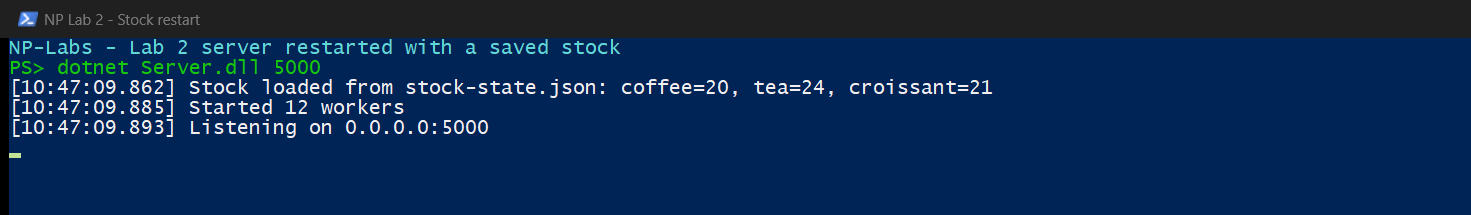
\includegraphics[width=0.9\linewidth]{figures/lab2-stock.png}
\caption{Console capture of a restarted C\# server loading the saved stock before it
accepts clients.}
\label{fig:stock}
\end{figure}

\section{Discussion}
\label{sec:discussion}

\subsection{Queueing and Little's law}

For the two-desktop run the throughput is 0.44 orders/s and the mean queue wait is
1.05~s. The four waits add up to about 16.8~s. The run lasted $16/0.44 \approx 36.4$~s,
so the time-average number of orders waiting is $16.8/36.4 \approx 0.46$. This equals
$\lambda W_q = 0.44 \times 1.05 \approx 0.46$, which is Little's law. The phone run
agrees in the same way ($0.57 \times 1.23 \approx 0.70$). Both sides are computed from
the same log, so the agreement checks the bookkeeping, not the model.

\subsection{Utilisation and Amdahl's law}

Amdahl's law describes the speed-up when part of the work is serial. Here
the limit is the number of workers, not the processor, because the preparation is a
wait. In the two-desktop run each worker was busy for one or two orders of about 4.2~s
in a run of about 36~s, so the utilisation is 12 to 23\%. The workers are mostly idle,
and the utilisation figures describe the simulated workload, not processor load.

\subsection{Timing overshoot}

Each prepared order took longer than its nominal time: about 0.2~s longer in the
two-desktop run and 0.36 to 0.59~s longer in the phone run (Figure~\ref{fig:prep}). The
overshoot grows with the number of \texttt{Thread.Sleep} calls. A 4~s coffee makes 40 calls
of 100~ms, and a 6~s order makes 60. The overshoot per call is about 5 to 10~ms, which is
consistent with the coarse timer of Windows. This is an inference from the measured times;
the timer itself was not measured.

\subsection{Admission control}

The order queue is unbounded in the C\# server, so a producer never blocks. The stock is
the real admission control: each accepted order consumes stock, and the stock is finite
until the provider delivers more. If the provider disconnects, the shop continues with the
stock it has, as the sheet requires. A bounded queue would give stronger backpressure, which
is listed as future work.

\section{Control Questions}
\label{sec:control}

The control questions of the sheet are answered here. Where a task question already
gives the full answer, the answer below refers to it.

    \subsubsection{1. What is the difference between the listening socket and the sockets returned by \texttt{accept}? How many of each does your server have with five clients and the provider?}
    The listening socket is bound to the port and is never used to send data. Each
    \texttt{accept} returns a new connected socket for one client, identified by the
    four-tuple of addresses and ports. With five clients and one provider the server has
    one listening socket and six accepted sockets, seven in total.

    \subsubsection{2. Why is one send not one receive? How does your protocol deal with it?}
    TCP has no message boundaries (Task~1, Q1). The protocol uses one JSON object per
    newline, and the server buffers the bytes until each line is complete.

    \subsubsection{3. What does it mean when \texttt{receive} returns 0? And when it fails because the connection was reset?}
    Zero means that the other side closed the connection in an orderly way. A reset means
    that the connection was aborted, for example by a killed process or a network error.
    In both cases the client is gone, and the server cancels its orders and returns their
    products (Task~4, Q1).

    \subsubsection{4. Where in your server is a producer--consumer pattern? Name the producers, the consumers, and the queue between them.}
    The producers are the connection threads, which validate orders and take products from
    the stock. The consumers are the workers, which take orders from the queue and prepare
    them. The queue is an unbounded \texttt{BlockingCollection} of \texttt{Order} objects in
    the C\# server; the Go server uses a channel with room for 1000 orders.

    \subsubsection{5. What does it cost when a thread waits for a client? What would change with 1000 clients?}
    Each waiting thread holds a stack, which reserves on the order of a megabyte of virtual
    memory, and each wake-up costs a context switch. With 1000 clients the server would have
    1000 threads, most of them idle. An asynchronous or event-driven model (for example
    \texttt{async}/\texttt{await} or \texttt{epoll}) would serve the same clients with far
    fewer threads.

    \subsubsection{6. Explain step by step a race condition that could happen on your server without its locks.}
    See Task~2, Q2: two threads read the last croissant, both decide that it is available,
    and both decrement the stock. Two clients receive one product, and the stock becomes
    negative.

    \subsubsection{7. What identifies one TCP connection? How can five clients on the same machine all be connected to the same port of the server?}
    A TCP connection is identified by the four-tuple of client address, client port, server
    address, and server port. Each client gets its own ephemeral source port, so the five
    connections differ in their client port, and the server accepts all five on port 5000.

\section{Conclusion and Future Work}
\label{sec:conclusion}

The coffee shop covers the four tasks and the three bonuses. The archived runs support the
queueing behaviour of Task~2, the cross-device protocol, the refund of an order that a worker
was preparing (Task~4), and stock persistence in both servers. The provider alerts (Task~3)
are supported by the code and the checklist, and the cancellation of an order that is still
queued by the code alone; neither has an archived run.

Future work follows from these gaps. The first item is an archived run that triggers a
low-stock alert, reconnects the provider, and cancels an order that is still queued. Beyond
that, the server could use an asynchronous or event-driven model to avoid the per-connection
thread cost; a bounded queue with backpressure instead of relying only on the
stock; heartbeats to detect silent network losses; richer per-order tracing and latency
histograms; a larger evaluation with more clients, repeated runs, and confidence intervals; and
a secure deployment with TLS and authenticated clients. The stock persistence could also be
extended to queued orders, so that they survive a crash.

\section{Evidence files}
\label{app:evidence}

\begin{table}[!ht]
\centering
\small
\begin{tabularx}{\textwidth}{@{}>{\raggedright\arraybackslash}p{0.44\textwidth} X@{}}
\toprule
Evidence & Content \\
\midrule
\path{Lab2/evidence/cross-device-2026-11-26/} & phone run: 16 Go clients and a provider, server CSV/JSON, charts; five-client C\# run in \path{desktop-csharp-clients-metrics/} \\
\path{Lab2/evidence/two-desktop-2026-11-26/} & two-desktop run: 16 Go clients and a provider, server metrics, transcripts; five-client C\# run in \path{windows-csharp-clients-metrics/}; disconnect run in \path{server-metrics-cancel/} and \path{server-cancel-run.txt} \\
\path{Lab2/evidence/stock-persistence-2026-11-26/} & C\# and Go restart tests with the stock before and after each step, logs, and client transcripts \\
\path{Lab2/report/report.pdf} & this report \\
\path{Lab2/KNOWLEDGE.md} & notes of the manual runs (20 clients, last-item race, mid-order disconnect, provider disconnect, server death) \\
\path{docs/tutorials/01-launch.md} & launch tutorial with screenshots \\
\path{docs/tutorials/02-testing.md} & defence and testing checklist \\
\bottomrule
\end{tabularx}
\caption{Where to find the raw evidence for this report.}
\end{table}

\section{Source Code and Build Instructions}\label{sec:source}

The complete source code is in the NP-Labs repository, in the 2 folder:
\begin{center}
\large
\url{https://github.com/Prince-of-Nothing/NP-Labs}
\end{center}

\begin{terminalwindow}[]
dotnet build Lab2/csharp/Server/Server.csproj
dotnet build Lab2/csharp/Client/Client.csproj
dotnet run --project Lab2/csharp/Server/Server.csproj -- 5000
dotnet run --project Lab2/csharp/Client/Client.csproj -- 127.0.0.1 5000 client
dotnet run --project Lab2/csharp/Client/Client.csproj -- 127.0.0.1 5000 provider
\end{terminalwindow}

The repository also has a one-command build for all labs: run \texttt{scripts/build-all.ps1}
in PowerShell (Windows) or \texttt{./scripts/build-all.sh} (Linux/macOS). It publishes the C\#
projects and builds the Go and Rust binaries, including the phone arm64 binaries, under
\texttt{dist/}. The charts are regenerated with \path{Lab2/scripts/metrics_report.py}.

\end{document}
